現在,我們對處理器高效使用的理解是:首先,CPU可以同時做多個操作,比如:同時做加法和乘法。不使用這種能力就是暴殄天物。此外,限制效率最大化能力的因素是,生成數據的速度,以供給這些操作進行計算。受到數據依賴關係的約束:如果一個操作計算了下一個操作用作輸入的值,那麼這兩個操作必須順序執行。處理這種依賴關係的方法是流水線操作,當執行循環或長的代碼序列時,處理器將交叉計算(如循環迭代),只要有可以獨立執行的操作即可。

使用流水線也有前提條件。流水線的\textbf{前提條件}:為了從循環迭代中交叉執行代碼,必須知道將執行什麼代碼。與上一節中瞭解到的信息進行比較,為了並行執行指令,必須預先知道輸入值。現在,為了在流水線中運行指令,必須知道指令是什麼。現在知道嗎?因為運行的代碼通常依賴於數據,每次遇到\texttt{if(條件)}語句時,要麼執行\texttt{true}分支,要麼執行\texttt{false}分支,但是在確定\textit{條件}之前我們並不知道會執行到哪個分支。像數據依賴是指令級並行的障礙一樣,條件執行或分支也是流水線的障礙。

隨著流水線的中斷,程序的效率會顯著降低。我們可以使用基準測試來觀察這種有害影響,例如不要寫這樣的代碼:

\begin{lstlisting}[style=styleCXX]
a1 += p1[i] + p2[i];
\end{lstlisting}

可以這樣寫:

\begin{lstlisting}[style=styleCXX]
a1 += (p1[i]>p2[i]) ? p1[i] : p2[i];
\end{lstlisting}

現在我們將數據依賴重新引入到代碼中了:

%\hspace*{\fill} \\ %插入空行
\begin{center}
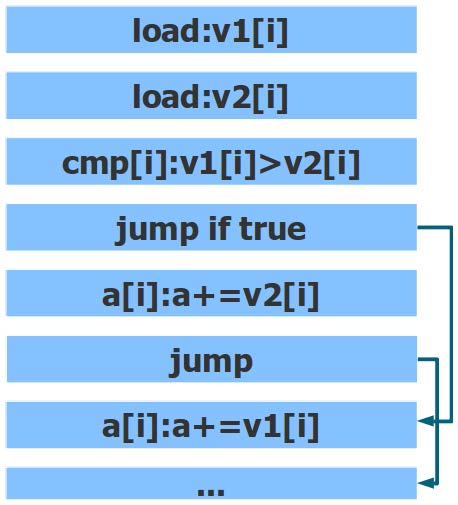
\includegraphics[width=0.4\textwidth]{content/1/chapter3/images/18.jpg}\\
圖3.18 - 轉移指令對流水線的影響
\end{center}

沒有好方法將這段代碼轉換為要執行的線性指令流,並且需要處理不能避免的條件跳轉。

實際情況要複雜一些,基準測試可能會出現性能的顯著下降,也可能不會。原因是許多處理器都有某種\textbf{條件移動}功能,甚至是\textbf{條件添加}指令,編譯器可以決定是否使用。如果發生這種情況,代碼就會變得完全有序,沒有跳轉或分支,並且可以完美地流水線化:

%\hspace*{\fill} \\ %插入空行
\begin{center}
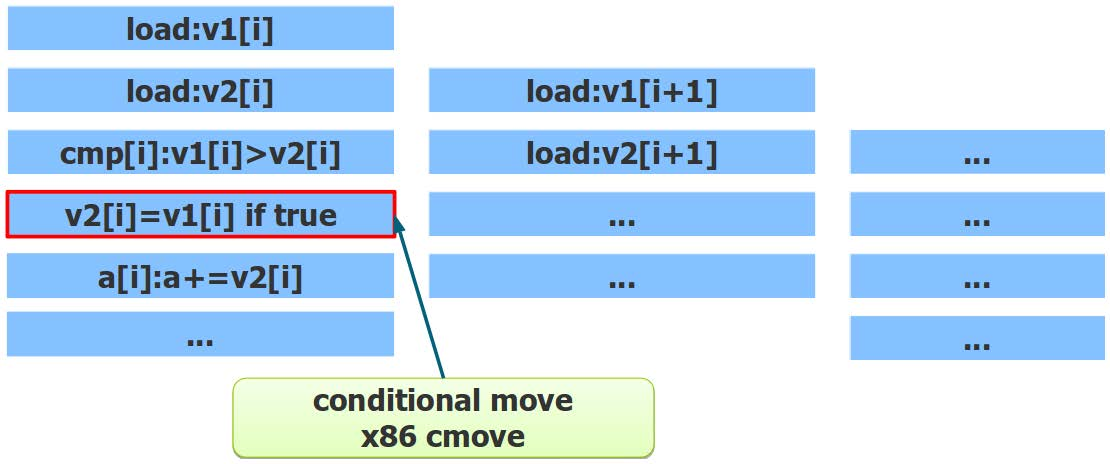
\includegraphics[width=0.9\textwidth]{content/1/chapter3/images/19.jpg}\\
圖3.19 - cmove將分支流水線化
\end{center}

x86的CPU有一個條件移動指令\texttt{cmove}(雖然不是所有編譯器都使用它來實現\texttt{?:}三元操作符)。具有AVX或AVX2指令集的處理器具有一組強大的掩碼加法和乘法指令,這些指令也可以用於實現一些條件代碼。這就是為什麼在用分支對代碼進行基準測試和優化時,需要檢查生成的目標代碼,並確認代碼中確實包含分支,以及確定是否影響了性能。還有一些分析器工具可用,我們稍後介紹。

雖然分支和條件在大多數現實程序中無處不在,但當程序減少到只有幾行代碼時就會消失,原因是編譯器可能使用了前面提到的條件指令。構造糟糕的基準測試的另一個原因是,編譯器能夠在編譯時計算出條件的值,大多數編譯器將完全優化代碼,比如:\texttt{if (true)}或\texttt{if (false)}生成的代碼中就沒了這個語句,永遠不會執行的代碼也會消除。要了解分支對循環流水線的有害影響,必須構造一個編譯器無法預測條件檢查結果的測試,可以從實際使用的程序中提取了一個數據集。下一個演示,將使用隨機值:

\hspace*{\fill} \\ %插入空行
\noindent
\textbf{02\_branch.C}
\begin{lstlisting}[style=styleCXX]
std::vector<unsigned long> v1(N), v2(N);
std::vector<int> c1(N);
for (size_t i = 0; i < N; ++i) {
	v1[i] = rand();
	v2[i] = rand();
	c1[i] = rand() & 1;
}
unsigned long* p1 = v1.data();
unsigned long* p2 = v2.data();
int* b1 = c1.data();
for (auto _ : state) {
	unsigned long a1 = 0, a2 = 0;
	for (size_t i = 0; i < N; ++i) {
		if (b1[i]) {
			a1 += p1[i];
		} else {
			a1 *= p2[i];
		}
	}
	benchmark::DoNotOptimize(a1);
	benchmark::DoNotOptimize(a2);
	benchmark::ClobberMemory();
}
\end{lstlisting}

同樣,有兩個輸入數組\texttt{v1}和\texttt{v2},以及一個隨機值為0和1的控制數組\texttt{c1}(這裡請避免使用\texttt{vector<bool>},它不是字節數組,而是一個打包的位數組,因此訪問它的開銷會很高,而且我們現在對位操作指令的基準測試不感興趣)。編譯器無法預測下一個隨機數是奇數還是偶數,因此不可能進行優化。此外,我們檢查了生成的機器碼,並確認編譯器(x86上的Clang-11)使用一個簡單的條件跳轉實現了這個循環。為了有一個基線測試,我們將這個循環的性能與在每次迭代中進行無條件加法和乘法的循環進行比較:\texttt{a1 += p1[i]*p2[i]}。這個簡單的循環在每次迭代中都做加法和乘法,由於流水線的存在,我們可以自由地進行加法運算,與下一次迭代的乘法運算同時執行。另一方面,條件分支不能自由的執行:

%\hspace*{\fill} \\ %插入空行
\begin{center}
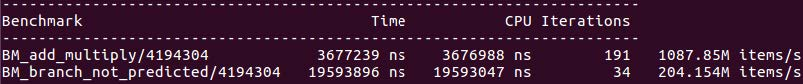
\includegraphics[width=0.9\textwidth]{content/1/chapter3/images/20.jpg}\\
圖 3.20
\end{center}

可以看到,條件代碼大約比順序代碼慢5倍。證實了我們的預測,當下一條指令依賴於上一條指令的結果時,代碼不能有效地流水化。

\subsubsubsection{3.5.1\hspace{0.2cm}分支預測}

聰明的讀者可能會指出,我們剛才描述的圖像可能不完整,甚至不是真實的。讓我們回到串行代碼上,例如:我們在上一節中使用的循環代碼:

\begin{lstlisting}[style=styleCXX]
for (size_t i = 0; i < N; ++i) {
	a1 += v1[i] + v2[i]; // s[i] = v1[i] + v2[i]
}
\end{lstlisting}

處理器視角的循環體:

%\hspace*{\fill} \\ %插入空行
\begin{center}
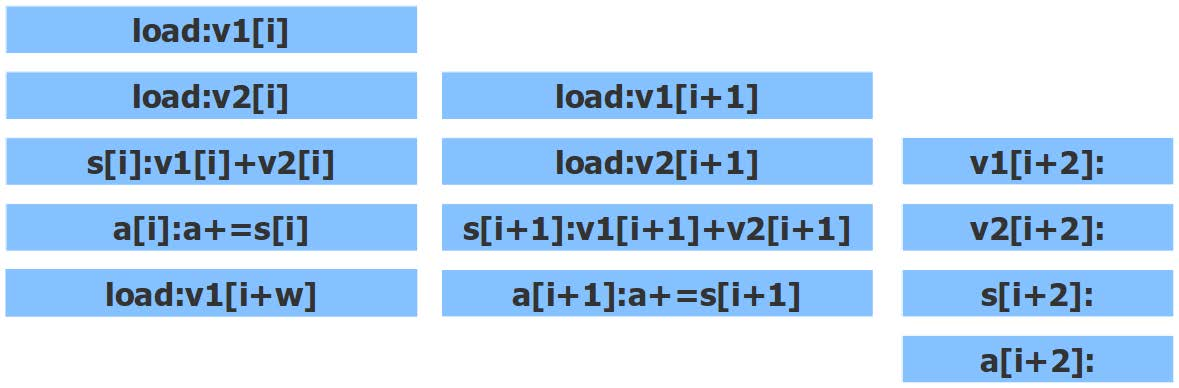
\includegraphics[width=0.8\textwidth]{content/1/chapter3/images/21.jpg}\\
圖3.21 - 寬度為w的流水線中執行的循環
\end{center}

圖3.21中,展示了三次交叉迭代,但可能有更多,流水線的總寬度是w,理想情況下,w足夠大。每個週期中,CPU執行指令都可以同時執行(這樣的峰值效率在實際中很少)。但請注意,在計算\texttt{p1[i] + p2[i]}的同時,可能不可能訪問\texttt{v[i+2]},因為不能保證循環有更多的兩次迭代,所以\texttt{v[i+2]}可能不存在,貿然訪問會導致未定義行為。前面代碼中有一個隱藏條件:每次迭代中,必須檢查i是否小於N,只有這樣才能執行第i次迭代的指令。

因此,在圖3.20中的比較是錯誤的,沒有將流水線的順序執行與不可預測的條件執行進行比較。實際上,這兩個基準測試都有分支。

真相介於兩者之間,我們瞭解條件執行的解決方案。流水線是數據依賴的解決方案,但分支戕害了它。分支存在時,保存流水線的方法是嘗試將條件代碼轉換為順序代碼,如果事先知道分支要走哪條路,就可以進行轉換。只需消除分支,然後繼續執行下一條指令。當然,如果事先知道情況如何,就沒必要這樣寫代碼了。這裡,考慮一下循環的終止條件。假設循環執行了很多次,可能條件\texttt{i < N}的計算結果為\texttt{true}(只有\texttt{1 / N}的機率會輸掉這個賭局)。

處理器使用\textbf{分支預測}技術進行押注。分析代碼中每一個分支的歷史,並假定該行為在未來不會變。循環結束後,處理器很快就會知道,大多數情況下,必須進行下一個迭代。因此,正確的做法是對下一次迭代進行流水線化。當然,必須將實際的結果寫入內存,直到計算條件確認迭代確實發生。處理器有一定數量的寫緩衝區來保存這些未確認的結果,然後再將它們提交到內存中。

因此,只添加了一個元素的循環流水,看起來與圖3.21所示完全一致。唯一的問題是,當第\texttt{i}次迭代完成之前開始執行迭代\texttt{i+2}時,處理器根據是否採用條件分支預測來下注的。這種確定代碼存在的執行方式,稱為\textbf{投機執行}。賭贏了,知道需要計算的時候,就可以獲取結果。如果輸了,必須放棄一些計算結果,以避免產生錯誤,例如:寫入內存新內容,覆蓋之前的內容,在大多數硬件平臺上無法撤消,而計算結果和將其存儲在寄存器中的過程完全可逆。當然,這會浪費我們的時間。

現在我們對流水線的工作原理有了更全面的瞭解。為了找到更多的指令並行執行,處理器要檢查循環的下一個迭代,並開始與當前迭代同時執行。該代碼包含一個條件分支,無法確切地知道將執行哪條指令,處理器根據過去檢查的結果進行有根據的猜測,並繼續推測執行該代碼。若這個預測正確,則流水線操作可以和無條件代碼一樣好。若預測錯誤,處理器必須丟棄預測得到的結果,獲取之前認為不需要的指令,並進行計算。這個事件稱為\textbf{刷新流水},是一個開銷很大的事件。

現在對圖3.20中的基準測試有了更好的理解,兩個循環都有檢查循環結束的條件。然而,預測幾乎是完美的,刷新流水只在循環的末端發生。條件基準測試也有基於隨機數的分支,\texttt{if(b1[i])},其中\texttt{b1[i]}有50\%的概率為真。處理器無法預測結果,並且一半的時間流水中斷了(或者更糟,如果設法欺騙了CPU,會使其做出了錯誤的預測)。

可以用實驗來驗證我們的理解,只需要把隨機條件改變成總是正確即可。唯一的問題是,我們必須以編譯器無法理解的方式來處理。常用的方法是將條件數組進行初始化:

\begin{lstlisting}[style=styleCXX]
c1[i] = rand() >= 0;
\end{lstlisting}

編譯器不知道函數\texttt{rand()}總是返回非負的隨機數,並且不會消除這種情況。CPU的分支預測器電路很快就會知道,如果\texttt{if(b1[i])}的值總是為真,那麼就會推測地執行相應的代碼。我們可以良好的預測分支和不準確預測分支的性能:

%\hspace*{\fill} \\ %插入空行
\begin{center}
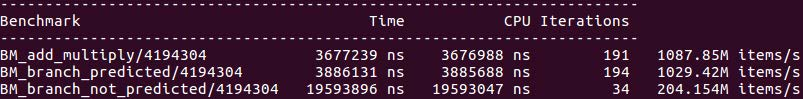
\includegraphics[width=0.9\textwidth]{content/1/chapter3/images/22.jpg}\\
圖 3.22
\end{center}

我們可以看到,良好預測分支的成本很低。

\subsubsubsection{3.5.2\hspace{0.2cm}錯誤預測分支的分析}

已經看到錯誤預測分支會對代碼性能產生多麼嚴重的影響,現在的問題是,如何找到這樣的代碼來優化?當然,包含這段代碼的函數所花費的時間比預期的要長,但是如何知道其原因是因預測錯誤的分支,還是其他原因才效率低下的呢?現在,我們已經瞭解了足夠多的知識,從而可以\textit{避免對性能的猜測},且猜測分支預測器的有效性挺沒趣的。通常,大多數分析器不僅可以分析執行時間,還可以分析決定效率的各種因素,包括分支預測失敗。

本章中,將再次使用perf分析器。第一步,運行這個分析器來收集基準程序的總體性能指標:

\begin{tcblisting}{commandshell={}}
$ perf stat ./benchmark
\end{tcblisting}

下面是隻運行\texttt{BM\_branch\_not\_predicted}基準測試的性能結果(其他基準測試註釋掉了):

%\hspace*{\fill} \\ %插入空行
\begin{center}
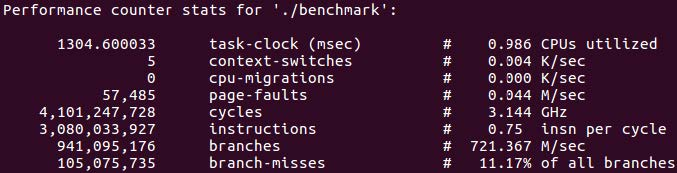
\includegraphics[width=0.9\textwidth]{content/1/chapter3/images/23.jpg}\\
圖3.23 - 預測分支失敗的基準測試數據
\end{center}

11\%的所有分支被預測錯誤(報告的最後一行)。請注意,這個數字是所有分支的累加,包括完全可預測的循環結束條件,因此11\%相當糟糕。我們應該將它與其他基準\texttt{BM\_branch\_predicted}進行比較,\texttt{BM\_branch\_predicted}和這個基準測試完全相同,只是條件總是為真:

%\hspace*{\fill} \\ %插入空行
\begin{center}
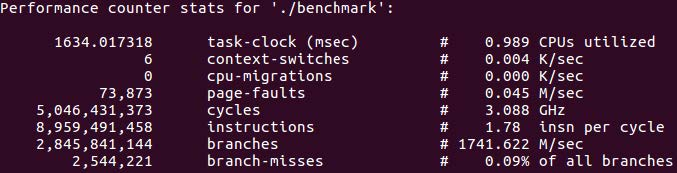
\includegraphics[width=0.9\textwidth]{content/1/chapter3/images/24.jpg}\\
圖3.24 - 具有預測良好分支的基準測試概要
\end{center}

這一次,不到0.1\%的分支沒有正確預測。

報告非常有用,可以用來強調或消除一些可能導致不良表現的原因。我們的案例中,可以得出結論,程序有一個或多個錯誤預測的分支。現在只需要找到是哪一個,分析器也可以幫忙查找。上一章中,使用分析器找出程序花費時間最多的地方,可以生成分支預測的逐行數據。我們只需要為分析器指定正確的性能計數器即可:

\begin{tcblisting}{commandshell={}}
$ perf record -e branches,branch-misses ./benchmark
\end{tcblisting}

我們的例子中,可以從\texttt{perf stat}的輸出複製計數器的名稱,因為它恰好是默認測量的計數器之一,完整的列表可以通過運行\texttt{perf -\,-list}獲得。

分析器運行程序並收集指標,可以通過生成數據報告來查看:

\begin{tcblisting}{commandshell={}}
$ perf report
\end{tcblisting}

報表分析器是交互式的,可以導航到每個函數的分支錯誤預測計數器:

%\hspace*{\fill} \\ %插入空行
\begin{center}
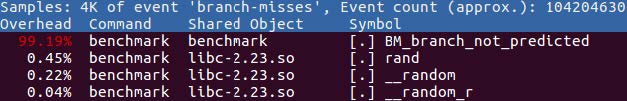
\includegraphics[width=0.9\textwidth]{content/1/chapter3/images/25.jpg}\\
圖3.25 - 錯誤預測分支的詳細報告
\end{center}

超過99\%的錯誤預測分支發生在一個函數中。因為函數很小,所以查找相應的條件運算應該不難。在更大的函數中,我們必須逐行查看概要信息。

現代處理器的分支預測硬件相當複雜,例如:函數從兩個不同的位置調用,當從第一個位置調用時,條件的計算結果為true,而從第二個位置調用時,相同的條件的計算結果為false,預測器會瞭解該模式,並根據函數調用正確地預測分支。類似地,預測器可以在數據中檢測出相當複雜的模式,例如:可以初始化我們的隨機條件變量,使值總是不可預測的,第一個是隨機的,但是下一個是與第一個相反的,以此類推:

\begin{lstlisting}[style=styleCXX]
for (size_t i = 0; i < N; ++i) {
	if (i == 0) c1[i] = rand() >= 0;
	else c1[i] = !c1[i - 1];
}
\end{lstlisting}

分析器確認該數據的分支預測率非常好:

%\hspace*{\fill} \\ %插入空行
\begin{center}
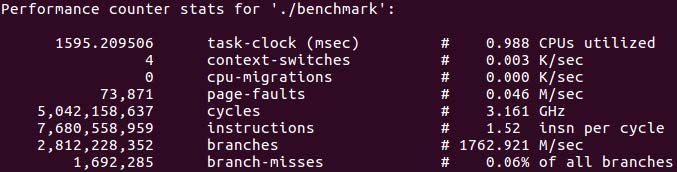
\includegraphics[width=0.9\textwidth]{content/1/chapter3/images/26.jpg}\\
圖3.26 - “真-假”模式的分支預測率
\end{center}

我們已經準備好如何高效使用處理器了。但必須承認,這裡忽略了一個很重要的問題。































